\chapter{System Overview \& Philosophy}
\label{ch:system_overview}

\section{Architectural Philosophy}
\label{sec:architectural_philosophy}

The \rus{} system embodies a \textbf{Multi-Layer Abstraction Architecture} (\textsc{MLAA}) that fundamentally separates concerns across distinct functional domains while maintaining tight integration through well-defined interfaces. This architectural philosophy enables several critical system properties:

\begin{description}
    \item[Domain Separation] Medical domain logic (USLib) is architecturally isolated from generic robotics functionality (TrajectoryLib), enabling independent evolution and specialized optimization.
    
    \item[Algorithmic Flexibility] Plugin-based algorithm selection with runtime configuration allows for adaptive performance optimization based on operational requirements.
    
    \item[Safety-First Design] Multi-level safety guarantees with graceful degradation ensure patient safety under all operational conditions.
    
    \item[Scalable Performance] Horizontal scaling through distributed computing patterns enables adaptation to diverse computational environments.
    
    \item[Clinical Compliance] Built-in validation and auditing capabilities facilitate regulatory compliance and quality assurance.
\end{description}

\subsection{Design Principles}

The \rus{} architecture adheres to six fundamental design principles:

\begin{enumerate}
    \item \textbf{Modularity}: Component-based architecture with clearly defined interfaces enabling independent development and testing of system components.
    
    \item \textbf{Extensibility}: Plugin architectures for algorithm and sensor integration facilitate system evolution and customization for specific clinical applications.
    
    \item \textbf{Reliability}: Redundant systems and graceful failure handling ensure continuous operation even under adverse conditions.
    
    \item \textbf{Performance}: Multi-threaded, cache-optimized implementations provide real-time performance guarantees required for clinical applications.
    
    \item \textbf{Maintainability}: Comprehensive logging, monitoring, and diagnostic capabilities enable efficient system maintenance and troubleshooting.
    
    \item \textbf{Interoperability}: Standards-compliant interfaces (DICOM, HL7 FHIR, ROS) ensure seamless integration with existing healthcare infrastructure.
\end{enumerate}

\section{System Taxonomy}
\label{sec:system_taxonomy}

The \rus{} system can be taxonomically classified as a \textbf{Hybrid Autonomous Robotic Medical Device} (\textsc{HARMD}) with the following distinctive characteristics:

\subsection{Autonomy Classification}

\begin{table}[H]
\centering
\caption{RUS Autonomy Characteristics}
\label{tab:autonomy_classification}
\begin{tabular}{@{}p{3cm}p{4cm}p{6cm}@{}}
\toprule
\textbf{Autonomy Level} & \textbf{Classification} & \textbf{Description} \\
\midrule
\textbf{Operational} & Supervised Autonomy & Self-contained decision-making with human oversight \\
\textbf{Tactical} & Human-in-the-Loop & Strategic decisions require human validation \\
\textbf{Safety} & Fail-Safe Autonomous & Independent safety monitoring and emergency response \\
\textbf{Learning} & Adaptive Autonomous & Continuous improvement through experience \\
\bottomrule
\end{tabular}
\end{table}

\subsection{Medical Device Classification}

According to FDA guidelines, the \rus{} system falls under:

\begin{itemize}
    \item \textbf{Class II Medical Device}: Moderate risk level requiring 510(k) premarket notification
    \item \textbf{Software as Medical Device} (SaMD): Class B - Non-serious healthcare decisions
    \item \textbf{Robotic-Assisted Surgery} considerations for autonomous operation
\end{itemize}

\section{Core System Capabilities}
\label{sec:core_capabilities}

\subsection{Automated Trajectory Planning}

The \rus{} implements advanced trajectory planning capabilities through multiple algorithmic approaches:

\begin{description}
    \item[\stomp{} Optimization] Stochastic trajectory optimization with parallel processing, achieving computational complexity of $O(K \times N \times M)$ where:
    \begin{align}
        K &= \text{Number of noisy trajectories (typically 4-20)} \\
        N &= \text{Trajectory discretization points (50-200)} \\
        M &= \text{Cost evaluation complexity (variable)}
    \end{align}
    
    \item[RRT* Planning] Rapidly-exploring Random Tree variants with asymptotic optimality guarantees
    
    \item[Informed RRT*] Heuristic-guided exploration for improved convergence rates
    
    \item[Hauser Planning] Dynamic programming approaches for time-optimal trajectory generation
\end{description}

\subsection{Real-time Collision Avoidance}

Collision detection and avoidance utilize hierarchical spatial data structures:

\begin{equation}
    \text{Query Time} = O(\log n + k)
\end{equation}

where $n$ represents the number of geometric primitives and $k$ denotes the number of collision candidates.

The \bvh{} tree implementation provides:
\begin{itemize}
    \item Surface Area Heuristic (SAH) construction for optimal tree structure
    \item Parallel tree traversal for multi-threaded collision queries
    \item Signed Distance Field (SDF) generation for gradient-based optimization
    \item Conservative advancement for continuous collision detection
\end{itemize}

\subsection{Force-Controlled Scanning}

Cartesian impedance control ensures safe patient interaction:

\begin{equation}
    \bm{F} = \bm{K}_c(\bm{x}_d - \bm{x}) + \bm{D}_c(\dot{\bm{x}}_d - \dot{\bm{x}})
\end{equation}

where:
\begin{align}
    \bm{F} &= \text{Applied force vector} \\
    \bm{K}_c &= \text{Cartesian stiffness matrix} \\
    \bm{D}_c &= \text{Cartesian damping matrix} \\
    \bm{x}_d, \bm{x} &= \text{Desired and actual end-effector positions}
\end{align}

\section{Hierarchical System Architecture}
\label{sec:hierarchical_architecture}

The \rus{} architecture implements a five-layer hierarchical structure, as illustrated in Figure \ref{fig:system_architecture}.

\begin{figure}[H]
\centering
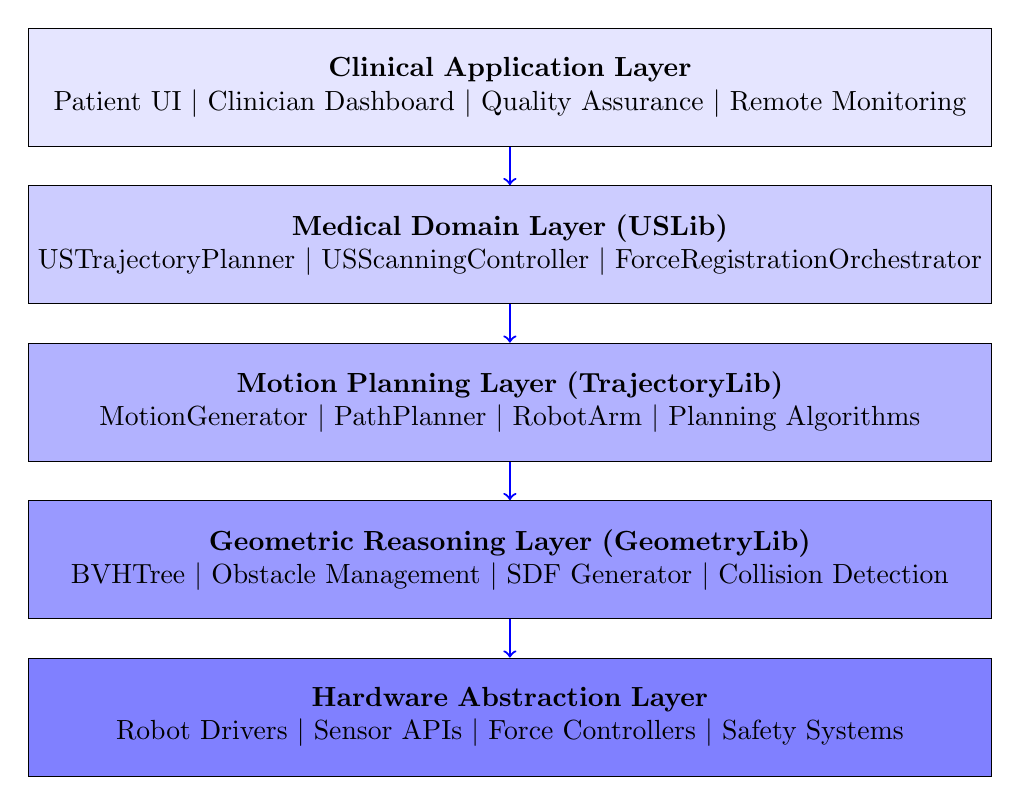
\begin{tikzpicture}[
    layer/.style={rectangle, draw, fill=blue!20, text width=12cm, text centered, minimum height=1.5cm},
    arrow/.style={->, thick, blue}
]

% Draw layers
\node[layer, fill=blue!10] (clinical) at (0,8) {\textbf{Clinical Application Layer}\\Patient UI $|$ Clinician Dashboard $|$ Quality Assurance $|$ Remote Monitoring};

\node[layer, fill=blue!20] (medical) at (0,6) {\textbf{Medical Domain Layer (USLib)}\\USTrajectoryPlanner $|$ USScanningController $|$ ForceRegistrationOrchestrator};

\node[layer, fill=blue!30] (motion) at (0,4) {\textbf{Motion Planning Layer (TrajectoryLib)}\\MotionGenerator $|$ PathPlanner $|$ RobotArm $|$ Planning Algorithms};

\node[layer, fill=blue!40] (geometry) at (0,2) {\textbf{Geometric Reasoning Layer (GeometryLib)}\\BVHTree $|$ Obstacle Management $|$ SDF Generator $|$ Collision Detection};

\node[layer, fill=blue!50] (hardware) at (0,0) {\textbf{Hardware Abstraction Layer}\\Robot Drivers $|$ Sensor APIs $|$ Force Controllers $|$ Safety Systems};

% Draw arrows
\draw[arrow] (clinical.south) -- (medical.north);
\draw[arrow] (medical.south) -- (motion.north);
\draw[arrow] (motion.south) -- (geometry.north);
\draw[arrow] (geometry.south) -- (hardware.north);

\end{tikzpicture}
\caption{RUS Hierarchical System Architecture}
\label{fig:system_architecture}
\end{figure}

\subsection{Layer Descriptions}

\paragraph{Clinical Application Layer}
Provides user interfaces and clinical workflow integration:
\begin{itemize}
    \item Patient interaction interfaces with guided positioning
    \item Clinician dashboards for system monitoring and control
    \item Quality assurance modules for automated validation
    \item Remote monitoring capabilities for multi-site deployment
\end{itemize}

\paragraph{Medical Domain Layer (USLib)}
Implements ultrasound-specific functionality:
\begin{itemize}
    \item \texttt{USTrajectoryPlanner}: Orchestrates multi-segment scanning trajectories
    \item \texttt{USScanningController}: Manages real-time scanning execution
    \item \texttt{ForceRegistrationOrchestrator}: Coordinates force-based positioning
\end{itemize}

\paragraph{Motion Planning Layer (TrajectoryLib)}
Provides advanced robotics algorithms:
\begin{itemize}
    \item \texttt{MotionGenerator}: \stomp{} and time-optimal trajectory generation
    \item \texttt{PathPlanner}: High-level path planning with multiple algorithms
    \item \texttt{RobotArm}: Kinematic modeling and constraint management
\end{itemize}

\paragraph{Geometric Reasoning Layer (GeometryLib)}
Implements spatial data structures and algorithms:
\begin{itemize}
    \item \texttt{BVHTree}: Hierarchical collision detection with $O(\log n)$ performance
    \item \texttt{Obstacle}: Generic obstacle representation and manipulation
    \item \texttt{STLProcessor}: Mesh processing and geometric computations
\end{itemize}

\paragraph{Hardware Abstraction Layer}
Provides device-independent hardware interfaces:
\begin{itemize}
    \item Robot control drivers with real-time guarantees
    \item Sensor integration APIs for multi-modal feedback
    \item Force control systems with safety monitoring
    \item Emergency stop and fault detection mechanisms
\end{itemize}

\section{Information Flow Architecture}
\label{sec:information_flow}

The \rus{} system implements a \textbf{Hierarchical Information Processing Model} with multiple concurrent data streams:

\subsection{Data Stream Classifications}

\begin{description}
    \item[Command Flow] Top-down directive propagation from clinical interface to hardware actuators with priority-based scheduling
    
    \item[Sensor Fusion] Multi-modal data integration including visual, force, and proprioceptive feedback with temporal synchronization
    
    \item[Feedback Loops] Real-time state monitoring and correction with adaptive control parameters
    
    \item[Event Propagation] Asynchronous event handling across architectural layers with publish-subscribe patterns
    
    \item[Audit Trails] Comprehensive logging for medical compliance with immutable data structures
\end{description}

\subsection{Real-time Performance Requirements}

The system maintains strict timing constraints across different operational modes:

\begin{table}[H]
\centering
\caption{Real-time Performance Requirements}
\label{tab:timing_requirements}
\begin{tabular}{@{}lccc@{}}
\toprule
\textbf{System Component} & \textbf{Update Rate} & \textbf{Deadline} & \textbf{Priority} \\
\midrule
Force Control Loop & 1 kHz & 1 ms & Critical \\
Collision Monitoring & 500 Hz & 2 ms & High \\
Trajectory Execution & 100 Hz & 10 ms & High \\
Safety Monitoring & 1 kHz & 1 ms & Critical \\
UI Updates & 60 Hz & 16.7 ms & Normal \\
Data Logging & 100 Hz & 10 ms & Low \\
\bottomrule
\end{tabular}
\end{table}

\section{Key System Properties}
\label{sec:system_properties}

\subsection{Safety Properties}

The \rus{} system implements multiple safety mechanisms:

\begin{enumerate}
    \item \textbf{Hardware Safety Interlocks}
    \begin{itemize}
        \item Emergency stop circuits with redundant monitoring
        \item Force limiting with configurable thresholds
        \item Workspace boundary enforcement
        \item Collision detection with immediate response
    \end{itemize}
    
    \item \textbf{Software Safety Monitors}
    \begin{itemize}
        \item Real-time trajectory validation
        \item Joint limit monitoring with soft and hard boundaries
        \item Velocity and acceleration constraint enforcement
        \item Fault detection and isolation algorithms
    \end{itemize}
    
    \item \textbf{Graceful Degradation}
    \begin{itemize}
        \item Adaptive performance scaling under computational load
        \item Alternative algorithm selection for failed components
        \item Safe system shutdown procedures
        \item Data preservation under fault conditions
    \end{itemize}
\end{enumerate}

\subsection{Performance Properties}

\begin{description}
    \item[Computational Scalability] Near-linear performance scaling with available computational resources through dynamic thread pool management
    
    \item[Memory Efficiency] Cache-optimized data structures with Structure-of-Arrays patterns and object pooling for high-frequency allocations
    
    \item[Real-time Guarantees] Hard real-time constraints for safety-critical components with deterministic execution paths
    
    \item[Adaptive Optimization] Dynamic algorithm parameter adjustment based on system performance metrics and operational requirements
\end{description}

\subsection{Reliability Properties}

\begin{itemize}
    \item \textbf{Fault Tolerance}: Comprehensive exception handling with recovery mechanisms
    \item \textbf{Data Integrity}: Checksums and validation for critical data structures
    \item \textbf{State Consistency}: Atomic operations and transactional updates
    \item \textbf{Diagnostic Capabilities}: Extensive logging and performance monitoring
\end{itemize}
